\chapter{Market Risk}
\label{chap:MarketRisk}

\section{Market Risk}



\section{Market Risk Metrics}

\section{The Computational Burden of Market Risk Computations}

\section{Market Risk as a Supervised Machine Learning Problem} {\label{sec:MktRisk_SML}}

\section{Model Scores for Market Risk}

\section{Unsupervised Machine Learning Alternatives}
\subsection{Deep Learning}
\subsection{Differential Deep Learning}
\subsection{Other}

\newpage

\section{A Base Case Example}

As a base case example we consider an option for which a closed form solution exists. This allows us compare the results obtained by a supervised machine learning algorithm to those obtained by the closed form formula.

In order to add both nonlinear features and the possibility of increasing the dimension of the problem, we will use a call option on the geometric mean of a basket.

\begin{equation}\label{eq:geom_digital}
\begin{aligned}
&V_{T}=\max\left(G_T-k,0\right) \\
&G_{T}=\left(\prod_{j=1}^{m} \frac{S_{T}^{j}}{S_{0}^{j}}\right)^{1 / m} \\
\end{aligned}
\end{equation}

Where $S_t^1,\ldots,S_t^m$ represent the prices of the underlying assets as of time t and $G_T$ represents the geometric mean of one plus the return of the different assets from time $0$ to time $T$. $T$ represents the option's payoff date.

We assume geometric Brownian motion dynamics \johan{Entiendo que esto no será la primera vez que aparezcan ecuaciones similares de finanzas matemáticas. La primera vez habría que citar alguna referencia.} \luis{Dejo en este punto de la t\'esis la referencia. Si hubiera ecuaciones de este tipo antes, mover\'ia dicha referencia.} for the different underlying assets under the risk neutral measure \footnote{A good reference regarding stochastic calculus applied to quentitative finance and derivatives pricing theory can be found here \cite{Borj}}:

\begin{equation}\label{eq:geom_brownianmotion}
\frac{S_{T}^{j}}{S_{t}^{j}}=\exp\left(\left(r-q_{j}-\frac{\sigma_{j}^{2}}{2}\right) \left( T - t\right)+\sigma_{j} \left(W_{T}^{j}-W_{t}^{j}\right)\right)
\end{equation}

Where $r$ represents the risk free rate, $q_j$ the continuous dividend yield , $\sigma_j$ the volatility and $W_T^j$ the change experienced form $0$ to $T$ of a Brownian motion. The $j$ index help us distinguish the parameters of the different underlying assets.
\johan{Un par de tonterías, pero comentar que $r$ y las $q_j$ se asumen constantes? Y aunque se introduce la matriz de correlaciones abajo, quizás estaría bien comentar aquí que los $W_t^j$ son correlados? Lo segundo lo digo porque abajo dice "Notice that..." y para notar eso faltaría ese dato, aunque supongo que si no se dice nada por defecto habrá que asumir una estructura general de correlación.}\luis{Incluyo el siguiente texto como respuesta a tu sugerencia} We are assuming constant interest rates, dividends and volatilities. The different Brownian processes will be correlated with time independent correlations. Although these assumptions are simplistic from a pricing perspective, we make them for the base case example to have a simple closed form formula. We should also keep in mind that machine learning techniques perform well when the number of features increase, so that these techniques can be extended to more complex pricing frameworks. 

Taking into account \ref{eq:geom_brownianmotion}

\begin{equation}\label{eq:geom_digital_distrib}
\left(\prod_{j=1}^m\frac{S_{T}^{j}}{S_{0}^{j}}\right)^{\frac{1}{m}} =\left(\prod_{j=1}^m\frac{S_{t}^{j}}{S_{0}^{j}}\right)^{\frac{1}{m}}\exp\left(\frac{1}{m} \sum_{j=1}^{m}\left(r-q_{j}-\frac{\sigma_{j}^{2}}{2}\right) \left(T-t\right)+\frac{1}{m} \sum_{j=1}^{m} \sigma_{j} \left(W_{T}^{j}-W_{t}^{j}\right)\right) 
\end{equation}

Notice that $G_T$, conditional on $S_t^1,\cdots,S_t^m$ is log-normally distributed with parameters:



\begin{equation} 
\label{eq:geom_digital_distrib_params1}
\begin{aligned} 
& G_T|\mathcal{F}_t \eqdistr A \exp\left(\mu+\Sigma\phi\right)\\
& A = \left(\prod_{j=1}^m\frac{S_{t}^{j}}{S_{0}^{j}}\right)^{\frac{1}{m}} \\
&\mu = \frac{1}{m}\sum_{j=1}^{m}\left(r-q_{j}-\frac{\sigma_{j}^{2}}{2}\right)\left(T-t\right) \\   
& \Sigma=\frac{1}{m}\sqrt{\sigma^{\top} C_{w} \sigma}
\end{aligned}
\end{equation}
\johan{Errata en la ecuación para $\mu$: $T \mapsto (T-t)$}\luis{Corregida}

Where $\mathcal{F}_t$ the market filtration as of time $t$, $\sigma$ is a column vector containing the volatilities of the different underlying assets, $C_W$ the covariance matrix of $W_T^1,\cdots,W_T^m$ and $\phi$ is a standard normal distributed random variable.
\johan{Va según gustos, pero conceptos matemáticos generales como $\eqdistr$, mover su definición al glosario?}\luis{movido, de momento $\eqdistr$}

\begin{equation} \label{eq:geom_digital_distrib_params2}
\begin{aligned}
&\sigma=\left[\begin{array}{c}
\sigma_{1} \\
\vdots \\
\sigma_{m}
\end{array}\right] \\
&C_{w}=\left[\begin{array}{cccc}
\left(T-t\right) & \rho_{12} \left(T-t\right) & \cdots & \rho_{1 m} \left(T-t\right) \\
\vdots & \vdots & & \vdots \\
\rho_{m 1} \left(T-t\right) & \rho_{m 2} \left(T-t\right) & \cdots &  \left(T-t\right)
\end{array}\right]
\end{aligned}
\end{equation} 

$\rho_{ij}$ represents the correlation of $W_t^i$ and $W_t^j$.

Given the distribution of $G_T$, the pricing formula as of time $t<T$ will be given by:

$$
\begin{array}{lll}
V_{t}&=&\exp (-r(T-t)) E_{\mathbb{Q}}\left[1_{\{G_{T}>K\}} | \mathcal{F}_t\right] \\
&& \\
&=&\left(A\exp\left(\mu+\frac{\Sigma^2}{2}\right)N\left(d_1\right)-k\left(d_2\right)\right)\exp\left(-r(T-t)\right)
\end{array}
$$

$$
\begin{aligned}
d_1 = \frac{\log\frac{A\exp\left(\mu+\frac{\Sigma^2}{2}\right)}{K}+\frac{\Sigma^2}{2}}{\Sigma} \\
d_2 = \frac{\log\frac{A\exp\left(\mu+\frac{\Sigma^2}{2}\right)}{K}-\frac{\Sigma^2}{2}}{\Sigma} \\
\end{aligned}
$$


% $$
% & E_{\mathbb{Q}}\left[1_{\{G_{T}>K\}} | \mathcal{F}_t\right]=P\left[Ae^{\mu+\sum \phi}>k\right] \\
% & =P\left[\phi<\frac{\log \frac{A}{K}+\mu}{\Sigma}\right]=N\left(\frac{\log \frac{A}{K}+\mu}{\Sigma}\right)
% \end{aligned}
% $$

Where $\phi$ represents a standard normal random variable and $N$ its cumulative distribution function. $\mathbb{Q}$ represents the risk neutral measure.


\subsection{Unhedged Portfolio}
 In this section we explore how the usage of machine learning techniques performs while trying to represent the payoff function in isolation. Nevertheless, we should keep in mind that it is common to perform market risk calculations for trading portfolios where exotics payoffs as the one introduced in the last section are hedged with vanilla instruments. This is the reason why in the next section we tackle the hedged portfolio case. 
 
 As payoff function we consider a call option on the geometric mean of a basket with two underlying assets $\{A,B\}$ with the following contract terms:
 
 \luis{Include more underlyings}  
 
\begin{center}
\begin{tabular}{||c | c||} 
 \hline
 Market risk horizon $(\Delta)$ & $10$ days \\ 
 \hline
 Time to maturity $(T-t-\Delta)$ & $3$ years \\
 \hline
 $S_0^A$ & $1.0$ \\
 \hline
 $S_0^B$ & $1.0$ \\
 \hline
 $K$ & $1.0$ \\
 \hline
 \end{tabular}
\end{center}

We assume the following values for market variables (model parameters) as the market risk base scenario:

\begin{center}
\begin{tabular}{||c | c||} 
 \hline
 $S_t^A$ & 1.0 \\
 \hline
 $S_t^B$ & 1.0 \\
 \hline
 $\sigma_t^A$ & $0.2$ \\
 \hline
 $\sigma_t^B$ & $0.3$ \\
 \hline
 $r$ & $0.01$ \\
 \hline
 $q_A$ & $0.0$ \\
 \hline
 $q_B$ & $0.0$ \\
 \hline
 $\rho$ & $0.8$ \\
 \hline
\end{tabular}
\end{center}

We apply market risk scenarios to $S_t^A,\ S_t^B,\ \sigma_t^A,\ \sigma_t^B$.
In order to apply market risk scenarios we make use of historical data for both the spot prices and the $1$ year \footnote{We are using the $1$ year implied volatility even though the product maturity is $3$ years due to better liquidity of the $1$ year maturity. In a real framework historical risk factors would be aligned with those used in pricing.} \johan{Not very important since this is an example, but mention why 1 year vol instead of 3 year vol?} \luis{Done as a footnote} implied at the money volatilities of BBVA and Santander from 2019-11-12 to 2021-10-11 (500 scenarios) \footnote{Source: Bloomberg}. We compute $10$ days log-normal overlapping returns from the historical data and apply these to our market risk variables $S_t^A,\ S_t^B,\ \sigma_t^A,\ \sigma_t^B$.

\luis{Use US stocks instead? Johan opinion?}
\johan{Could be interesting to include a case of less correlated stocks in the basket.}\luis{Pending}

In figure \ref{fig:distrib_P} we represent the $10$ days overlapping log returns of our historical data. By inspection of figure \ref{fig:distrib_P}, we can conclude that the historical shocks are not normally distributed.  

\begin{figure}[H] 
\centering
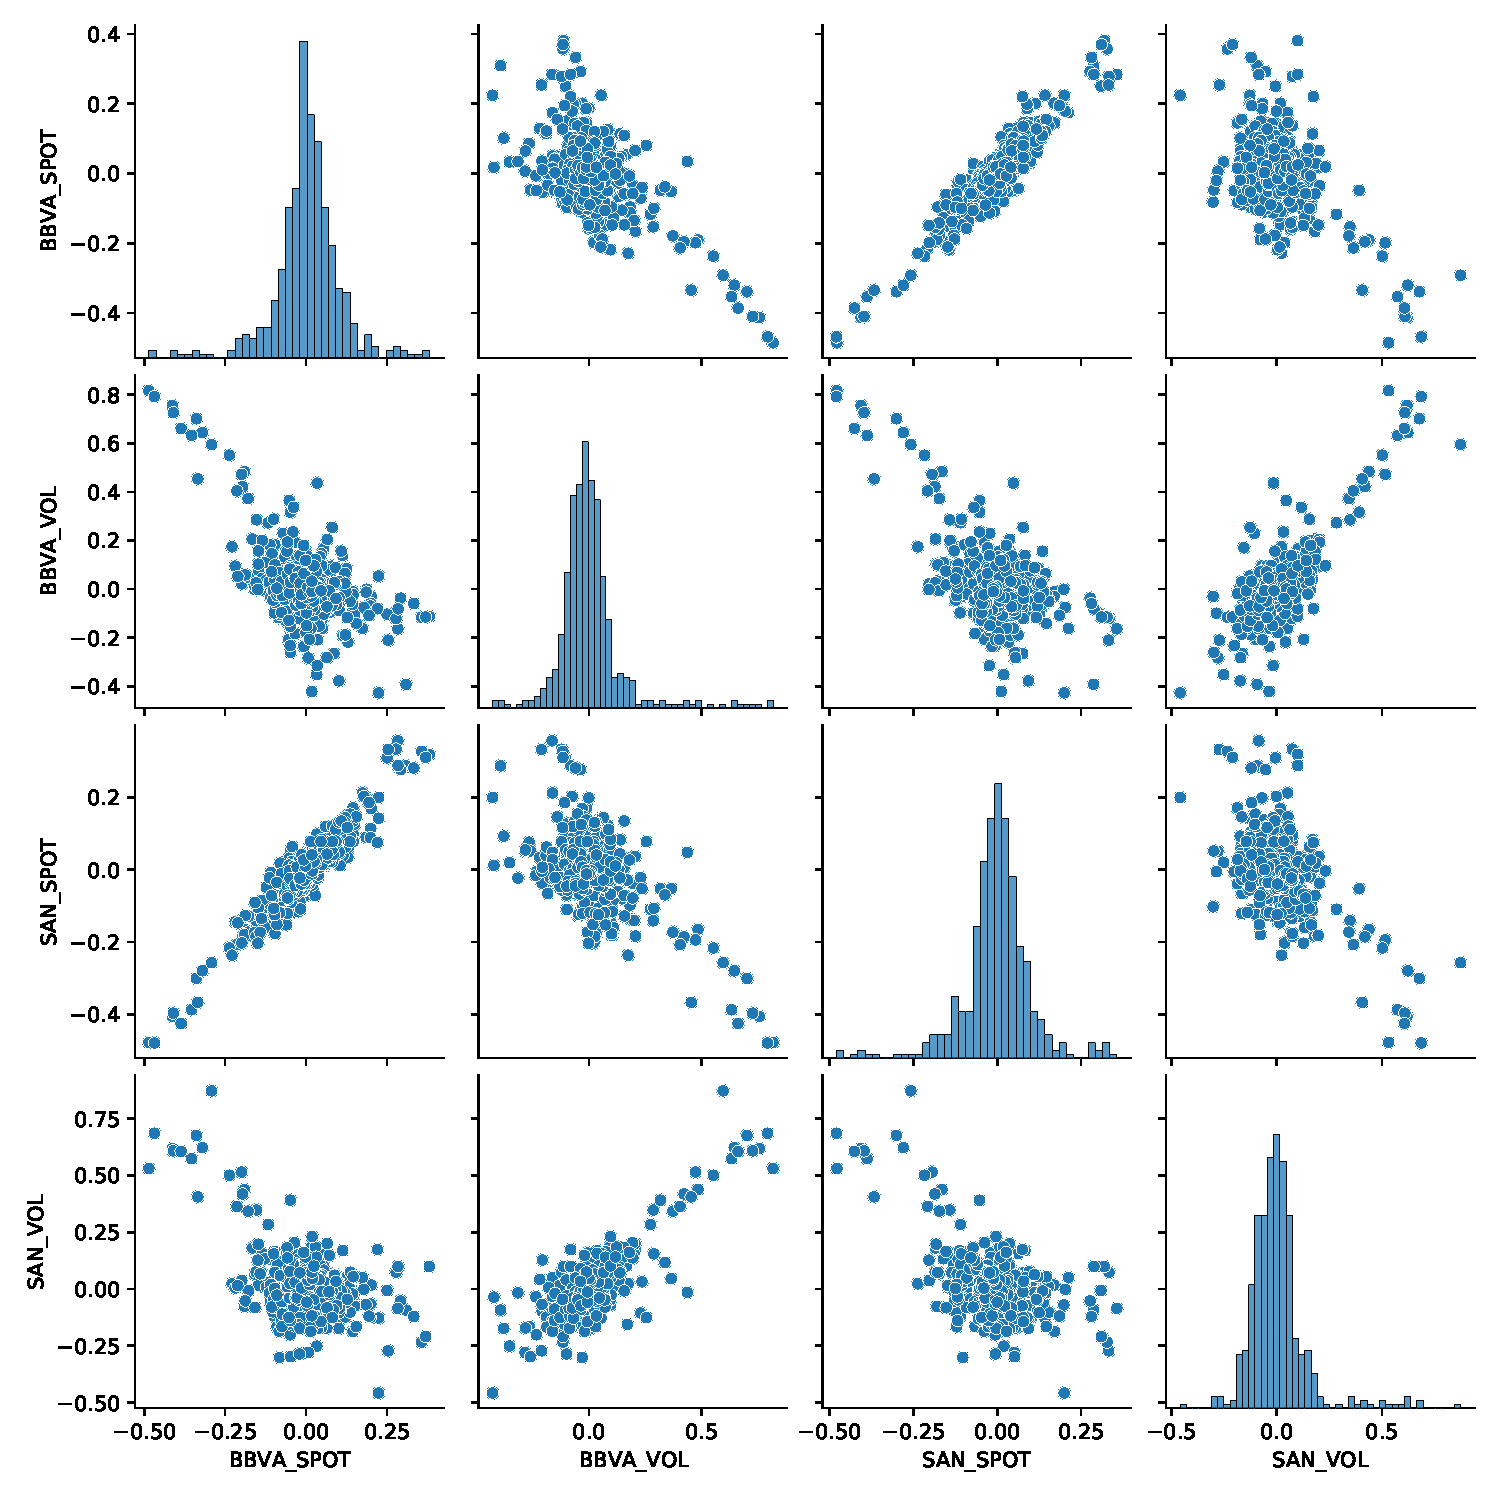
\includegraphics[width=1.0\textwidth]{Figures/MarketRisk/histdata.pdf}
\caption{Distribution of $10$ days log returns of market data. Marginal distributions of the different risk factors are plotted in the diagonal. Pairwise joint distributions are plotted in off diagonal figures.}
\label{fig:distrib_P}
\end{figure}

As already mentioned in section \ref{sec:MktRisk_SML}, historical data is scarce, so that in order to train a machine learning model we have to generate synthetic data distributed as the historical shocks. The task of obtaining the distribution behind data is part of the unsupervised machine learning paradigm. Generation of synthetic market data will be covered in chapter \ref{chap:Synthetic} of this thesis. In this section we will use a Gaussian Mixture with $5$ components in order to reflect the fact that our data is not normally distributed \footnote{We use the implementation in \href{https://scikit-learn.org/stable/modules/generated/sklearn.mixture.GaussianMixture.html}{Scikit Learn}}. We sample $100,000$ scenarios to train our models, $20,000$ to cross-validate them and $20,000$ scenarios to test the model that minimizes the score metric. We use the mean squared error as score metric.

\johan{This is very interesting! Maybe it fits somewhere else in the thesis, but it would also be very interesting to compare the results of what would be obtained if synthetic data were not used, and the model instead be trained (if possible) directly on the historical data.}\luis{The thing is that historical data is scarce (just 500 scenarios). Further explanation wrt this to be included in section 2.4. For the time being I have included a little bit more regarding the usage of the Gaussian Mixture in the previous paragraph}

\begin{figure}[H] 
\centering
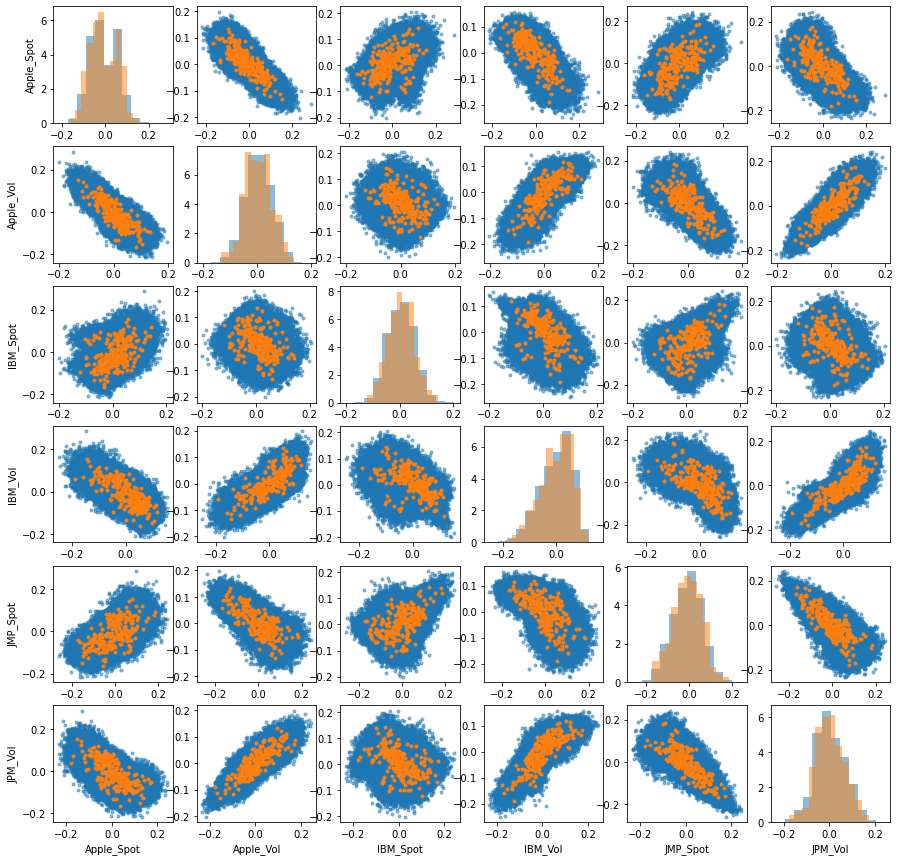
\includegraphics[width=1.0\textwidth]{Figures/MarketRisk/GaussMixture.png}
\caption{Marginal and joint distribution of both historical (blue) and synthetic shocks -simulated under the fitted Gaussian mixture model- (orange).}
\label{fig:distrib_P_simul}
\end{figure}
\johan{Entiendo que está pendiente, pero faltaría descripción de la figura.}\luis{Resuelto}

For each of these scenarios generated under the historical measure $\mathbb{P}$ that take us from $t$ (base scenario date) to $t+\Delta$, with $\Delta$ being the market risk horizon, we generate a single risk neutral scenario that takes us from $t+\Delta$ to $T$ (product maturity). These risk neutral scenarios are generated under \ref{eq:geom_brownianmotion}. 
\johan{No entiendo porqué los escenarios risk neutral van desde $t-\Delta$. Pensaría que o bien se asume que el tiempo no evoluciona, en el cálculo de riesgo de mercado, en cuyo caso el pricing va basado en evolución desde $t$ hasta $T$, bien se asume que evoluciona, y en tal caso el escenario base va desde $t$, mientras que los escenarios simulados van desde $t+\Delta$.}\luis{Ten\'ia una errata. Los escenarios risk neutral van de $t+\Delta$ a $T$. Errata corregida.} 

So that the features of our models will be comprised of:

$$
X^{(k)}=\left[\begin{array}{c}
S_{t+\Delta}^{A,(k)} \\ \\
S_{t+\Delta}^{B,(k)} \\ \\
\sigma_{t+\Delta}^{A,(k)} \\ \\
\sigma_{t+\Delta}^{B,(k)}
\end{array}\right], \ \  k=1, \ldots, n
$$

Where $(k)$ represents the $k$-th example and $n$ the number of examples.

With respect to the labels, these will be 

$$
y^{(k)}=\left[\begin{array}{l}
\tilde{V}_{T}^{(k)} \\ \\
\frac{\partial \tilde{V}_{T}^{(k)}}{\partial S_{t+\Delta}^{A,(k)}} \\ \\
\frac{\partial \tilde{V}_{T}^{(k)}}{\partial S_{t+\Delta}^{B,(k)}} \\ \\
\frac{\partial \tilde{V}_{T}^{(k)}}{\partial \sigma_{t+\Delta}^{A,(k)}} \\ \\
\frac{\partial \tilde{V}_{T}^{(k)}}{\partial \sigma_{t+\Delta}^{B,(k)}}
\end{array}\right],\ \ k=1, \ldots, n
$$

Where

$$\tilde{V}_{T}^{(k)} := V_T\left(S_T^{A.(k)}, S_T^{B.(k)}\right)\exp\left(-r\left(T-t-\Delta\right)\right)$$

$\frac{\partial \tilde{V}_{T}^{(k)}}{\partial S_{t+\Delta}^{A,(k)}},\  
\frac{\partial \tilde{V}_{T}^{(k)}}{\partial S_{t+\Delta}^{B,(k)}},\ 
\frac{\partial \tilde{V}_{T}^{(k)}}{\partial \sigma_{t+\Delta}^{A,(k)}},\ 
\frac{\partial \tilde{V}_{T}^{(k)}}{\partial \sigma_{t+\Delta}^{B,(k)}}
$ are path-wise derivatives computed with the help of algorithmic differentiation techniques\footnote{Path-wise derivatives have been computed with \href{www.Tensorflow.org}{Tensorflow} , same library has been used to train the deep learning models. }. Notice that these are only taken into account under the differential deep learning approach.

With respect to hyper-parameters related to the model architecture and its regularization, we use the following:

\luis{Path-wise differentials have been computed using Tensorflow. Should it be mentioned? Johan / Jorge opinion}

\jorge{Sí me parece interesante, creo que le da valor. No veo por qué no} \luis{Comentado en nota de pie de p\'agina}

\begin{center}
\begin{tabular}{||l | c||} 
 \hline
 Differential machine learning regularization parameter & $\{0.0, 0.1, 0.5, 1.0, 10.0\}$ \\
 \hline
 Number of cells in each hidden layer  & $\{32, 64, 128\}$  \\
 \hline
 Number of hidden layers  & $\{1 ,2 ,4 ,6\}$  \\
 \hline
 \end{tabular}
\end{center}


Notice that when we are using a differential machine learning regularization parameter of 0.0, we are using a feed-forward neural network with dense layers. We consider every combination of hyper-parameters, so that we end up with $60$ different models. With respect to hyper-parameters more related to training and not on the model architecture and its regularization:

\luis{In the FFNN, with no differential machine learning, we are not using regularization. Maybe I should include dropout layers. Nevertheless the implementation should be changed and try to generate sensitivities wrt inputs by algorithmic differentiation instead of doing the algorithmic differentiation / code transformation proposed in the paper.}

\begin{center}
\begin{tabular}{||l | c||} 
 \hline
 Number of epochs & $20$ \\
 \hline
 Mini batch size  & $32$  \\
 \hline
 Optimizer &  Adam(learning rate = 0.001, $\beta_1=0.9$,$\beta_2=0.999$,$\epsilon=1e-7$ ) \\
  \hline
 \end{tabular}
\end{center}
Both mini batch size and the optimizer hyper-parameters have been chosen in line with standard values. With respect to the number of epochs, its impact will be analyzed later. 

\johan{Any comment on how we do not expect the results to be sensitive to the fixed parameters?}\luis{De momento he puesto el p\'arrafo anterior. Quiz\'as debiera dar revisar este punto m\'as adelante}

Since we have a closed form formula for our pricing function, we can easily compute the Bayes error\footnote{Lowest possible error} by calculating the mean squared error between $\tilde{V}_{T}$ (noisy data) and $V_{t+\Delta}$ (closed form formula):
\johan{Te preguntaré sobre esto la próxima vez que hablamos porque no entiendo como defines el noisy data... lo mismo no estoy entendiendo bien el problema, pero porqué el error no es cero, por definición, si se usa la fórmula analítica?}\luis{Todo modelo de ML supervisado trata de generar $E\left[Y/X\right]$. Si $Y$ fuera la f\'ormula cerrada, o un MC convergido, esperar\'iamos que el error del modelo perfecto fuera cero. Aqu\'i, por aquello de evitar Montecarlo squared, cada escenario de riesgo de mercado tiene un \'unico escenario riesgo neutro, por ello es imposible llegar a un error 0. Es decir, condidionado a un escenario de riesgo de mercado, los flujos de caja riesgo neutro futuros representan dispersi\'on vs su valor medio. La idea es dar m\'as detalles sobre todo esto en secciones previas.}

$$\textbf{Bayes error}:=\frac{1}{N_{CV}}\sum_{j\in CV}\left(\tilde{V}_{T}^{(k)}-V_{t+\Delta}^{(k)}\right)^2$$

Obtaining a value of $0.109186$. $CV$ represents the set of cross validation examples, $N_{CV}$ the number of these and $V_{t+\Delta}^{(k)} := V\left(t+\Delta, S_{t+\Delta}^{A,(k)}
,S_{t+\Delta}^{B,(k)}
,\sigma_{t+\Delta}^{A,(k)}
\sigma_{t+\Delta}^{B,(k)}\right)$.

In figure \ref{fig:MSE_CV} we represent the mean squared error in the cross validation set of the different models together with the Bayes error. Notice that, as expected, the Bayes error is smaller that the errors produced by any of the models.

\johan{It is not easy to distinguish the different models. Is the best model with $\alpha = 1.0$ 2 hidden layers, 32 cells, or 6 hidden layers 128 cells? Maybe a higher res figure with different type of lines to distinguish similar colors?}
\johan{There is not a dramatic improvement when introducing the differentials... is this because the data set is (synthetically) very large? Or is it because the pricing function is effectively one-dimensional?}
\luis{Con respecto a las figuras: las he cambiado a formato pdf. Las ten\'ia en png y la calidad era mucho peor. Tambi\'en el detalle de que el texto en las figuras tenga la misma fuente q la t\'esis. Con respecto a los colores: es cierto q en el momento en que se ponen varios gr\'aficos los colores se confunden. Por aquello de no volverme loco poniendo colores a mano, los resultados obtenidos por el mejor modelo}
\luis{Con respecto a efecto de $\alpha$ incluyo m\'as comentarios.}

\begin{figure}[H] 
\centering
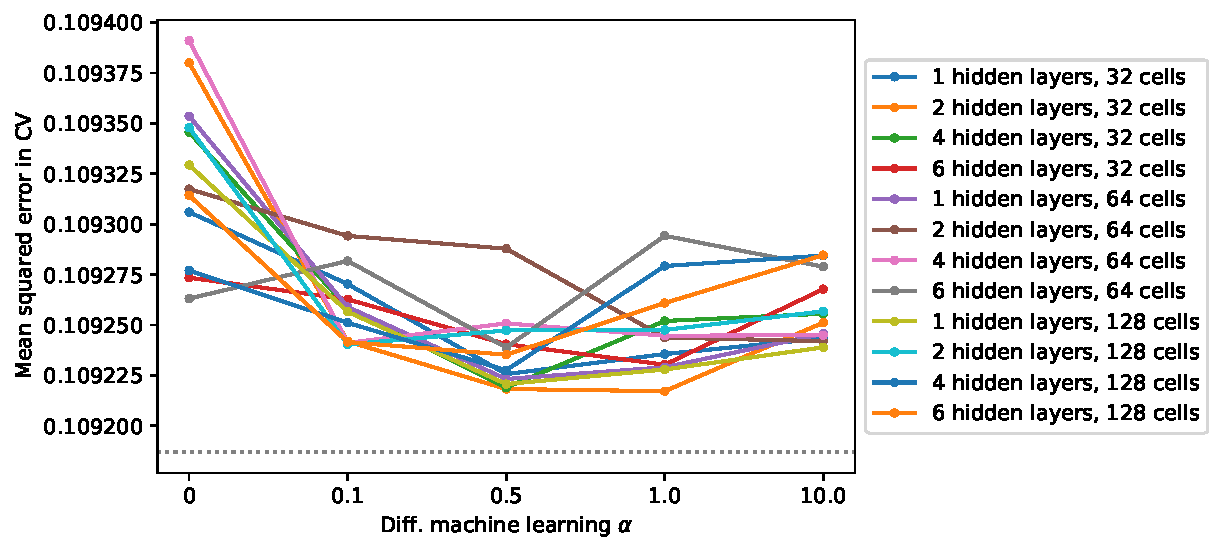
\includegraphics[width=1.0\textwidth]{Figures/MarketRisk/MSE_CV.pdf}
\caption{Mean squared error in the cross validation set of the different models together with the Bayes error (dotted line)}
\label{fig:MSE_CV}
\end{figure}

The best model in the cross validation set has the following hyper-parameters and scores:

\begin{center}
\begin{tabular}{||l | c||} 
 \hline
Differential machine learning regularization parameter & 1.0 \\
 \hline
Number of cells in each hidden layer &  32 \\
  \hline
Number of hidden cells &  32 \\
  \hline
Mean squared error train &  0.1059278 \\
  \hline
Mean squared error test &  0.109217 \\
  \hline
 \end{tabular}
\end{center}

In figure \ref{fig:MSE_CV_train_test} we have plotted the mean shared error as a function of the differential machine learning regularization parameter for every model under both the train and the cross validation sets. Bayes error is also represented. We observe the following:

\begin{itemize}
    \item For every model the train error is smaller than the Bayes error. Therefore we are suffering from variance.   
    \item The differential machine learning parameter does not help us reduce variance dramatically. This is in line with \cite{HugeSavine}, where they state that the differential machine learning technique is more in line with data augmentation than to regularization. This implies that together with the differential machine learning regularization term, it would be convenient to include a bias-variance controlling feature such as early stopping, dropout or $L1$ or $L2$ regularization.
\end{itemize}





\begin{figure}[H] 
\centering
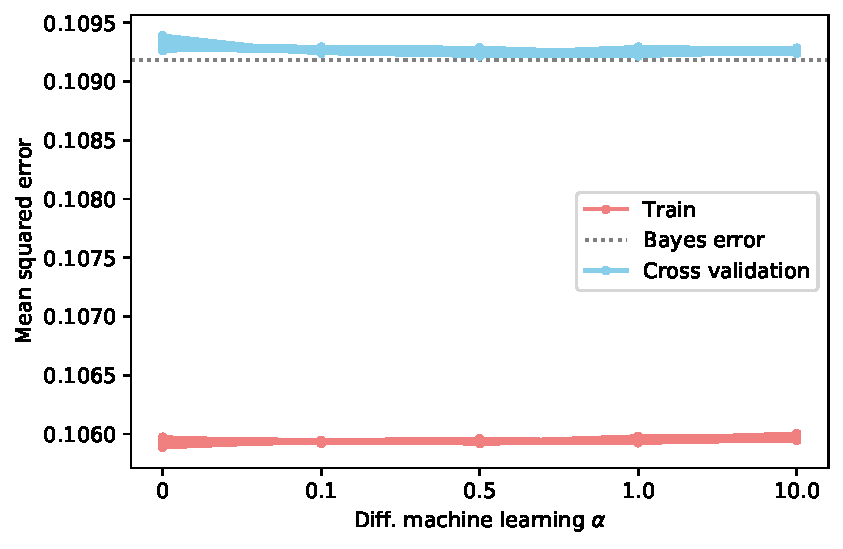
\includegraphics[width=1.0\textwidth]{Figures/MarketRisk/train_test_mse.pdf}
\caption{Mean squared error in train and cross validation sets together with Bayes error}
\label{fig:MSE_CV_train_test}
\end{figure}

\cite{dirac}

\cite{einstein}





\subsection{Hedged Portfolio Problem}
\subsection{Converged vs non Converged Y}
\subsection{Transfer Learning}





